%=========================================================
\chapter{Modelo de la interacción}	
\label{cap:modInteraccion}

Este capítulo describe ...

\section{Modelo de navegación}

La navegación entre pantallas se muestra en la figura~\ref{fig:mapa}. en el se explica ...\\

%\begin{figure}[htbp]
%	\begin{center}
	%		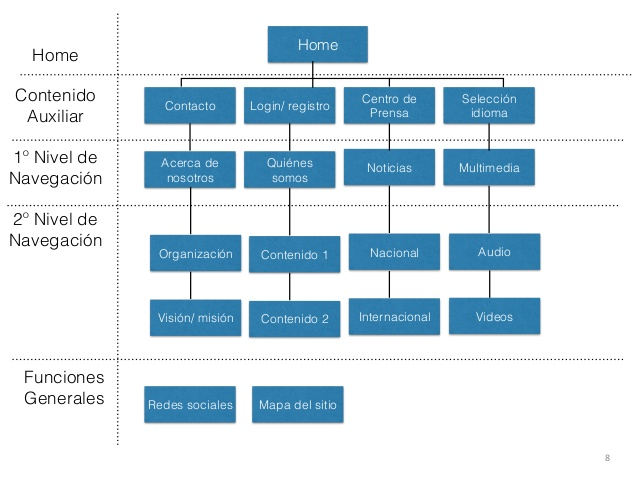
\includegraphics[width=.7\textwidth]{images/mapa}
	%		\caption{mapa}
	%		\label{fig:mapa}
	%	\end{center}
%\end{figure}

\newpage
% !TeX root = ../ejemplo.tex

%--------------------------------------
\subsection{IU01 Pantalla Iniciar sesión de personal escolar móvil} 

\subsubsection{Objetivo}
	Controlar el acceso al sistema mediante una contraseña a fin de que cada usuario acceda solo a las operaciones permitidas para su perfil.

\subsubsection{Diseño}
	Esta pantalla \IUref{IU01}{Pantalla Iniciar sesión de personal escolar móvil} (ver figura~\ref{IU01}) aparece al iniciar el sistema para los empleados. Para ingresar al mismo se debe escribir el RFC del empleado y la contraseña. 

\IUfig[.35]{UI-CU01}{IU01}{Pantalla Iniciar sesión de personal escolar móvil.}

\subsubsection{Salidas}

Saludo del sistema y mención de su nombre.

\subsubsection{Entradas}
En caso del empleado RFC, Contraseña y en caso del alumno CURP, Contraseña

\subsubsection{Comandos}
\begin{itemize}
	\item \IUbutton{Entrar}: Verifica que el empleado se encuentre registrado y la contraseña sea la correcta. Si la verificación es correcta, se verifica que tipo de empleado y se muestra la pantalla \IUref{IUE01}{Pantalla de Menús de docente} si es docente o \IUref{IUE02}{Pantalla de Menús de personal de seguridad} si es personal de seguridad.
	
	\item \IUbutton{Presiona aquí para pedir su activación}: Redirige a la pantalla \IUref{UI32}{Pantalla de Solicitar desbloqueo de cuenta}
	
\end{itemize}

\subsubsection{Mensajes}

\begin{Citemize}
	\item MSG-1 Los campos no están correctamente llenados. 
	\item MSG-2 Su cuenta esta bloqueada. 
	\item MSG-3 El RFC o la contraseña no corresponden con ningún empleado. 
	\item MSG-4 El proceso no se pudo realizar por un fallo de red. 
	\item MSG-5 Su cuenta ha sido bloqueada por la gran cantidad de intentos de inicio sesión fallidos.
\end{Citemize}


\newpage

% !TeX root = ../ejemplo.tex

%--------------------------------------
\section{IU02 Pantalla Consultar calendario escolar}

\subsection{Objetivo}
Permitir que los usuarios puedan ver el calendario escolar y pedir que se les recuerde cuantos días faltan para que el periodo de ETS comience.
\subsection{Diseño}
    Esta pantalla \IUref{IU02}{Pantalla Consultar calendario escolar} (ver figura~\ref{IU02}) puede ser accedida desde cualquier otra pantalla que no sea el inicio de sesión mediante el botón con forma de calendario.

\IUfig[.35]{UI-CU02}{IU02}{Pantalla Consultar calendario escolar.}

\IUfig[.5]{UI-CU02_2}{IU02-2}{Pantalla Consultar calendario escolar.}

\subsection{Salidas}

    Menciona cuantos días faltan para el periodo de ETS o si menciona que ya es periodo de ETS.

\subsection{Entradas}
   Ninguna.

\subsection{Comandos}
\begin{itemize}
    \item \IUbutton{Calcular cuantos días faltan para el periodo de ETS} toma el día actual y el día de inicio del periodo de ETS más cercano y calcula cuantos días faltan.
    \item \IUbutton{Campana} Redirige a la pantalla \IUref{UI03}{Consultar notificaciones}.
    \item \IUbutton{Home} Redirige a la pantalla de menú correspondiente al tipo de usuario.
\end{itemize}

\subsection{Mensajes}
     
\begin{Citemize}
    \item {\bf MSG7}{``Actualmente es periodo de ETS.''}

    \item {\bf MSG8}{``Actualmente el periodo de ETS no ha sido establecido.''}
\end{Citemize}


\newpage

% !TeX root = ../ejemplo.tex

%--------------------------------------
\section{IU03 Pantalla Consultar notificaciones}

\subsection{Objetivo}
Permitir que los usuarios puedan gestionar sus notificaciones y marcarlas como leidas.
\subsection{Diseño}
    Esta pantalla \IUref{IU03}{Pantalla Consultar notificaciones } (ver figura~\ref{IU03}) puede ser accedida desde cualquier otra pantalla que no sea el inicio de sesión mediante el botón con forma de campana.
\IUfig[.35]{UI-CU03}{IU03}{Pantalla Consultar notificaciones.}

\IUfig[.5]{UI-CU03_2}{IU03-2}{Pantalla Consultar notificaciones.}
\subsection{Salidas}
Menciona que la notificación seleccionada ha sido establecida como leída.
\subsection{Entradas}
   Ninguna.

\subsection{Comandos}
\begin{itemize}
    \item \IUbutton{Botón con palomita} toma la notificación seleccionada y la marca como leída.
    \item \IUbutton{Buscador} En este buscador se puede buscar las notificaciones por fecha.
    \item \IUbutton{Calendario} Redirige a la pantalla \IUref{UI02}{Consultar calendario escolar}
    \item \IUbutton{Home} Redirige a la pantalla de menú correspondiente al tipo de usuario.
\end{itemize}

\subsection{Mensajes}
     
\begin{Citemize}
    \item {\bf MSG9-}{``Actualmente no hay notificaciones.''} 
\end{Citemize}



\newpage

%--------------------------------------
\section{IU04}{Pantalla Periodo de ETS}

\subsection{Objetivo}
	Permitir al docente consultar los periodos de ETS que le han sido asignados. 

\subsection{Diseño}
	Esta pantalla \IUref{IU04}{Pantalla Periodo de ETS} (ver figura~\ref{IU04}) aparece luego de seleccionar la opción de Consultar Periodos de ETS de la pantalla principal. 

\IUfig[.35]{cu04}{IU04}{Pantalla Periodo de ETS.}

\subsection{Salidas}

	Lista de periodos de ETS asignados. 

\subsection{Entradas}
Ninguna

\subsection{Comandos}

\begin{Citemize}
	\item \IUbutton{Calendario} Redirige a la pantalla \IUref{UI02}{Consultar calendario escolar}.
	\item \IUbutton{Campana} Redirige a la pantalla \IUref{UI03}{Consultar notificaciones }.
	\item \IUbutton{Home} Redirige a la pantalla de bienvenida correspondiente al tipo de usuario.
	\item \IUbutton{Periodo de ETS} Selecciona un periodo de ETS y lo redirige a la \IUref{IU04}{pantalla Periodo de ETS}. 
\end{Citemize}


\subsection{Mensajes}

\begin{Citemize}
	\item {\bf MSG-9}{``Error al consultar la base de datos. Intente nuevamente más tarde''.}
	\item {\bf MSG-10}{``No tienes periodos de ETS asignados.''}
\end{Citemize}


\newpage

%--------------------------------------
\section{IU05 Pantalla Consultar ETS}

\subsection{Objetivo}
	Permitir al docente consultar los ETS que tiene asignados. 

\subsection{Diseño}
	Esta pantalla \IUref{IU05}{Pantalla Consultar ETS} (ver figura~\ref{IU05}) aparece luego de seleccionar un periodo de ETS. 

\IUfig[.35]{cu05}{IU05}{Pantalla Consultar ETS.}

\subsection{Salidas}
	Lista de ETS asignados. 

\subsection{Entradas}
	Ninguna
	
\subsection{Comandos}
\begin{Citemize}

	\item \IUbutton{Calendario} Redirige a la pantalla \IUref{UI02}{Consultar calendario escolar}.
	\item \IUbutton{Campana} Redirige a la pantalla \IUref{UI03}{Consultar notificaciones }.
	\item \IUbutton{Home} Redirige a la pantalla de bienvenida correspondiente al tipo de usuario.
	\item \IUbutton{ETS} Selecciona un ETS y lo redirige a la \IUref{IU06}{pantalla Información de ETS}.
\end{Citemize}

\subsection{Mensajes}

\begin{Citemize}
	\item {\bf MSG-9}{``Error al consultar la base de datos. Intente nuevamente más tarde.''.}
	\item {\bf MSG-11}{``No hay ETS asignados actualmente.''}
\end{Citemize}


\newpage

%--------------------------------------
\section{IU06 Pantalla Información de ETS}

\subsection{Objetivo}
	Permitir al docente visualizar la información detallada cada ETS que tiene asignados.
	
\subsection{Diseño}
	Esta pantalla \IUref{IU06}{Pantalla Información de ETS} (ver figura~\ref{IU06}) aparece luego de seleccionar un ETS asignado. 

\IUfig[.35]{cu06}{IU06}{Pantalla Información de ETS}

\subsection{Salidas}

	Información detallada del ETS seleccionado. 

\subsection{Entradas}
Ninguna

\subsection{Comandos}
\begin{itemize}
	\item \IUbutton{Ver alumnos} Redirige a la pantalla \IUref{IU06}{consultar lista de alumnos inscritos a un ETS}
\end{itemize}

\subsection{Mensajes}

\begin{Citemize}
	\item {\bf MSG-12}{``Información no disponible para el ETS seleccionado''}
	\item {\bf MSG-9}{``Error al consultar la base de datos. Intente nuevamente más tarde.''}
\end{Citemize}


\newpage

%%--------------------------------------
\section{IU07 Pantalla de Solicitar remplazo}

\subsection{Objetivo}
Permitir al docente pedir que otro docente lo remplaze en la aplicacion de un ETS.

\subsection{Diseño}
Esta pantalla \IUref{IU07}{Pantalla de Solicitar remplazo} (ver figura~\ref{IU07}) aparece luego de que el docente presione el boton \IUbutton{Solicitar docente ayudante} en la pantalla \IUref{IU06}{Pantalla Información de ETS}.

\IUfig[.35]{UI-CU43}{IU07}{Pantalla de Solicitar remplazo}

\subsection{Salidas}
Confirmación de envio de solicitud de remplazo del docente Y y se muestra {\bf MSG-13}{``La notificación ha sido mandada al jefe de departamento y/o al presidente de academia.''}

\subsection{Entradas}
Identificador del ETS y Razon por la que se pide el remplazo.

\subsection{Comandos}
\begin{itemize}
	\item \IUbutton{Enviar}: Permite enviar la notificación al jefe de departamento y/o al presidente de academia para pedir el remplazo.
	\item \IUbutton{Calendario} Redirige a la pantalla \IUref{UI02}{Consultar calendario escolar}.
    \item \IUbutton{Campana} Redirige a la pantalla \IUref{UI03}{Consultar notificaciones }.
    \item \IUbutton{Home} Redirige a la pantalla de bienvenida correspondiente al tipo de usuario.
\end{itemize}

\subsection{Mensajes}

\begin{Citemize}
	\item {\bf MSG-4}{``El proceso no se pudo realizar por un fallo de red.''}
	\item {\bf MSG-13}{``La notificación ha sido mandada al jefe de departamento y/o al presidente de academia.''}
\end{Citemize}


%\newpage

%--------------------------------------
\section{IU08 Pantalla Lista de asistencia de ETS}

\subsection{Objetivo}
Permitir al docente visualizar la asistencia de los alumnos inscritos a un ETS asignado.

\subsection{Diseño}
Esta pantalla aparece luego de registrar la asistencia de los alumnos en la \IUref{IU08}{Pantalla lista de asistencia de ETS} (ver figura~\ref{IU08})

\IUfig[.35]{cu08}{IU08}{Pantalla Lista de asistencia de ETS}

\subsection{Salidas}
Lista de asistencia de ETS.

\subsection{Entradas}
Ninguna

\subsection{Comandos}
\begin{itemize}
	\item \IUbutton{Alumno} Selecciona un alumno de la lista para registrar su asistencia y lo redirige a la pantalla \IUref{IU17}{reconocimiento facial}.
	\item \IUbutton{Calendario} Redirige a la pantalla \IUref{UI02}{Consultar calendario escolar}.
    \item \IUbutton{Campana} Redirige a la pantalla \IUref{UI03}{Consultar notificaciones }.
    \item \IUbutton{Home} Redirige a la pantalla de bienvenida correspondiente al tipo de usuario.
\end{itemize}

\subsection{Mensajes}

\begin{Citemize}
	\item {\bf MSG-16}{``No hay alumnos inscritos en este ETS.''}
	\item {\bf MSG-9}{``Error al consultar la base de datos. Intente nuevamente más tarde.''}
	\item {\bf MSG-18}{``Asistencia registrada exitosamente.''}  
\end{Citemize}
\newpage

%--------------------------------------
\subsection{IU09 Asignar docente de remplazo}

\subsubsection{Objetivo}
Permitir al jefe de departamento y/o al presidente de academia responder a las solicitudes de remplazo y asignar un docente de remplazo para el ETS especifico.

\subsubsection{Diseño}
Esta pantalla \IUref{IU09}{Asignar docente de remplazo} (ver figura~\ref{IU09}) aparece luego de que el jefe de departamento y/o al presidente de academia revisen sus notificaciones y seleccione una solicitud de remplazo.

\IUfig[.35]{UI-CU44}{IU09}{Pantalla de Asignar docente de remplazo}

\subsubsection{Salidas}
Confirmación de asignación del nuevo docente y se muestra el mensaje \bf MSG-42{``docente de remplazo asignado con exito.''}.

\subsubsection{Entradas}
Identificador del ETS y nombre del nuevo docente asignado.

\subsubsection{Comandos}
\begin{itemize}
	\item \IUbutton{Asignar}: Permite enviar la notificación docente de que su remplzado ha sido asignado y ademas asigna el remplazo como docente aplicador en el sistema.
\end{itemize}

\subsubsection{Mensajes}

\begin{Citemize}
	\item {\bf MSG-28} {``El proceso no se pudo realizar por un fallo de red''.}
	\item {\bf MSG-42}{``docente de remplazo asignado con exito'.'}
\end{Citemize}



\newpage


%--------------------------------------
\section{IU10 Pantalla Código QR}

\subsection{Objetivo}
Permitir al personal de seguridad escanear el código QR de la credencial del alumno.

\subsection{Diseño}
Esta pantalla \IUref{IU10}{Pantalla Código QR} (ver figura~\ref{IU10}) aparece una vez que el personal de seguridad active la función de escanear credencial del menú. 

\IUfig[.35]{cu12}{IU10}{Pantalla Código QR}

\subsection{Salidas}
Información del alumno

\subsection{Entradas}
Ninguna

\subsection{Comandos}
\begin{itemize}
	\item \IUbutton{Escanear}: Permite escanear el código QR de la credencial del alumno.
	\item \IUbutton{Calendario} Redirige a la pantalla \IUref{UI02}{Consultar calendario escolar}.
    \item \IUbutton{Campana} Redirige a la pantalla \IUref{UI03}{Consultar notificaciones }.
    \item \IUbutton{Home} Redirige a la pantalla de bienvenida correspondiente al tipo de usuario.
\end{itemize}

\subsection{Mensajes}

\begin{Citemize}
	\item {\bf MSG-9}{``Error al consultar la base de datos. Intente nuevamente más tarde.''}.
	\item {\bf MSG-20}{``Alumno no registrado. Verifique el código QR o intente nuevamente.''}
	\item {\bf MSG-19}{``Código QR ilegible. Intente nuevamente.''}
\end{Citemize}


\newpage

%--------------------------------------
\section{IU11}{Pantalla Credencial del alumno}

\subsection{Objetivo}
	Permitir al personal de seguridad consultar la información del alumno mediante el escaneo del código QR de su credencial.

\subsection{Diseño}
Esta pantalla aparece luego de que se escanea el código QR de la credencial del alumno \IUref{IU11}{Pantalla Credencial del alumno} (ver figura~\ref{IU11}).
	

\IUfig[.35]{cu14}{IU11}{Pantalla Credencial del alumno}

\subsection{Salidas}
	Información del alumno

\subsection{Entradas}
Ninguna

\subsection{Comandos}
\begin{itemize}
	\item \IUbutton{Registrar asistencia}: Permite registrar la asistencia del alumno.
	\item \IUbutton{Calendario} Redirige a la pantalla \IUref{UI02}{Consultar calendario escolar}.
    \item \IUbutton{Campana} Redirige a la pantalla \IUref{UI03}{Consultar notificaciones }.
    \item \IUbutton{Home} Redirige a la pantalla de bienvenida correspondiente al tipo de usuario.
\end{itemize}

\subsection{Mensajes}

\begin{Citemize}
	\item {\bf MSG-20}{``Alumno no registrado''}
	\item {\bf MSG-11}{``Error al consultar la base de datos. Intente nuevamente más tarde.''}
\end{Citemize}


\newpage

%--------------------------------------
\section{IU12-1 Pantalla Buscar alumno por boleta}

\subsection{Objetivo}
	Permitir al personal de seguridad buscar la información de un alumno utilizando su numero de boleta. 

\subsection{Diseño}
	Esta pantalla \IUref{IU12}{Pantalla Buscar alumno} (ver figura~\ref{IU12}) aparece luego de seleccionar la opción Consultar alumno. 

\IUfig[.35]{cu11}{IU12}{Pantalla Buscar alumno.}

\subsection{Salidas}
	Información del alumno.

\subsection{Entradas}
Número de boleta del alumno. 

\subsection{Comandos}
Buscador: Permite al usuario buscar al alumno ingresando su numero de boleta. 

\subsection{Mensajes}

\begin{Citemize}
	\item {\bf MSG-20-}{``Alumno no registrado''}
\end{Citemize}


\newpage

%%--------------------------------------
\section{IU12-2 Pantalla Buscar alumno por nombre}

\subsection{Objetivo}
Permitir al personal de seguridad buscar la información de un alumno utilizando su nombre. 

\subsection{Diseño}
Esta pantalla \IUref{IU12}{Pantalla Buscar alumno} aparece luego de seleccionar la opción Consultar alumno. 

\IUfig[.35]{cu11}{IU12}{Pantalla Buscar alumno.}

\subsection{Salidas}
Información del alumno.

\subsection{Entradas}
Nombre del alumno. 

\subsection{Comandos}

\begin{itemize}

	\item Buscador: Permite al usuario buscar al alumno ingresando su nombre. 
	\item \IUbutton{Calendario} Redirige a la pantalla \IUref{UI02}{Consultar calendario escolar}.
    \item \IUbutton{Campana} Redirige a la pantalla \IUref{UI03}{Consultar notificaciones }.
    \item \IUbutton{Home} Redirige a la pantalla de bienvenida correspondiente al tipo de usuario.
\end{itemize}

\subsection{Mensajes}

\begin{Citemize}
	\item {\bf MSG-20}{``Alumno no registrado''}
\end{Citemize}



%\newpage

%--------------------------------------
\subsection{IU13 Pantalla consultar lista de alumnos inscritos a un ETS}

\subsubsection{Objetivo}
Permitir al docente visualizar la lista de los alumnos inscritos a un ETS asignado.

\subsubsection{Diseño}
Esta pantalla aparece luego de seleccionar un ETS en la \IUref{IU13}{Pantalla Informacion de ETS} (ver figura~\ref{IU06} y muestra la boleta, el nombre completo y la foto de los alumnos inscritos al ETS)

\IUfig[.35]{cu07}{IU13}{Consultar lista de alumnos inscritos a un ETS}

\subsubsection{Salidas}
Lista de los alumnos inscritos al ETS.

\subsubsection{Entradas}
Ninguna

\subsubsection{Comandos}
\begin{itemize}
    \item \IUbutton{Calendario} Redirige a la pantalla \IUref{UI02}{Consultar calendario escolar}.
    \item \IUbutton{Campana} Redirige a la pantalla \IUref{UI03}{Consultar notificaciones }.
    \item \IUbutton{Home} Redirige a la pantalla de bienvenida correspondiente al tipo de usuario.
	\item \IUbutton{Tomar asistencia} redirige a la pantalla \IUref{IU08}{Lista de asistencia de ETS}.
\end{itemize}

\subsubsection{Mensajes}

\begin{Citemize}
	\item {\bf MSG-14}{``No hay alumnos inscritos en este ETS.''}
	\item {\bf MSG9-}{``Error al consultar la base de datos. Intente nuevamente más tarde.''}. 
\end{Citemize}
\newpage

%--------------------------------------
\section{IU14} {Pantalla Periodo de ETS del alumno}

\subsection{Objetivo}
	Permitir al alumno consultar los periodos de ETS que le han sido asignados. 

\subsection{Diseño}
	Esta pantalla \IUref{IU14}{Pantalla Periodo de ETS del alumno} (ver figura~\ref{IU14}) aparece luego de seleccionar la opción de Consultar Periodos.

\IUfig[.35]{cu16}{IU14}{Pantalla Periodo de ETS del alumno.}

\subsection{Salidas}
	Lista de periodos de ETS. 

\subsection{Entradas}
Ninguna

\subsection{Comandos}

\begin{itemize}
	\item \IUbutton{Calendario} Redirige a la pantalla \IUref{UI02}{Consultar calendario escolar}.
	\item \IUbutton{Campana} Redirige a la pantalla \IUref{UI03}{Consultar notificaciones }.
	\item \IUbutton{Home} Redirige a la pantalla de bienvenida correspondiente al tipo de usuario.
	\item \IUbutton{Periodo de ETS} Selecciona un periodo de ETS y lo redirige a la pantalla \IUref{UI15}{consultar ETS del alumno}.
\end{itemize}

\subsection{Mensajes}

\begin{Citemize}
	\item {\bf MSG-25}{``No hay periodos de ETS''}
	\item {\bf MSG-9}{``Error al consultar la base de datos. Intente nuevamente más tarde.''}
\end{Citemize}


\newpage

%--------------------------------------
\section{IU15} {Pantalla Consultar ETS del alumno}

\subsection{Objetivo}
Permitir al alumno consultar los ETS que tiene inscritos. 

\subsection{Diseño}
Esta pantalla \IUref{IU15}{Pantalla Consultar ETS del alumno} (ver figura~\ref{IU15}) aparece luego de seleccionar un periodo de ETS. 

\IUfig[.35]{cu17}{IU15}{Pantalla Consultar ETS del alumno.}

\subsection{Salidas}
Lista de ETS asignados. 

\subsection{Entradas}
Ninguna


\subsection{Comandos}

\begin{itemize}
	\item \IUbutton{Calendario} Redirige a la pantalla \IUref{UI02}{Consultar calendario escolar}.
	\item \IUbutton{Campana} Redirige a la pantalla \IUref{UI03}{Consultar notificaciones }.
	\item \IUbutton{Home} Redirige a la pantalla de bienvenida correspondiente al tipo de usuario.
\end{itemize}
\subsection{Mensajes}

\begin{Citemize}
	\item {\bf MSG-26}{``No hay ETS inscritos actualmente.''}
	\item {\bf MSG-09}{``Error al consultar la base de datos. Intente nuevamente más tarde.''}
\end{Citemize}

\newpage

%%--------------------------------------
\section{IU15} {Pantalla Consultar ETS del alumno}

\subsection{Objetivo}
Permitir al alumno consultar los ETS que tiene inscritos. 

\subsection{Diseño}
Esta pantalla \IUref{IU15}{Pantalla Consultar ETS del alumno} (ver figura~\ref{IU15}) aparece luego de seleccionar un periodo de ETS. 

\IUfig[.35]{cu17}{IU15}{Pantalla Consultar ETS del alumno.}

\subsection{Salidas}
Lista de ETS asignados. 

\subsection{Entradas}
Ninguna


\subsection{Comandos}

\begin{itemize}
	\item \IUbutton{Calendario} Redirige a la pantalla \IUref{UI02}{Consultar calendario escolar}.
	\item \IUbutton{Campana} Redirige a la pantalla \IUref{UI03}{Consultar notificaciones }.
	\item \IUbutton{Home} Redirige a la pantalla de bienvenida correspondiente al tipo de usuario.
\end{itemize}
\subsection{Mensajes}

\begin{Citemize}
	\item {\bf MSG-26}{``No hay ETS inscritos actualmente.''}
	\item {\bf MSG-09}{``Error al consultar la base de datos. Intente nuevamente más tarde.''}
\end{Citemize}

%--------------------------------------
\section{IU16 Pantalla Información de ETS}

\subsection{Objetivo}
Permitir al alumno visualizar la información detallada cada ETS que tiene inscrito.

\subsection{Diseño}
Esta pantalla \IUref{IU16}{Pantalla de Información de ETS del alumno} (ver figura~\ref{IU16}) aparece luego de seleccionar un ETS inscrito. 

\IUfig[.35]{cu18}{IU16}{Pantalla de Información de ETS del alumno}

\subsection{Salidas}

Información detallada del ETS seleccionado. 

\subsection{Entradas}
Ninguna


\subsection{Comandos}
\begin{itemize}
	\item \IUbutton{Calendario} Redirige a la pantalla \IUref{UI02}{Consultar calendario escolar}.
    \item \IUbutton{Campana} Redirige a la pantalla \IUref{UI03}{Consultar notificaciones }.
    \item \IUbutton{Home} Redirige a la pantalla de bienvenida correspondiente al tipo de usuario.
\end{itemize}

\subsection{Mensajes}

\begin{Citemize}
	\item {\bf MSG-13}{``Información no disponible para el ETS seleccinado''}
	\item {\bf MSG-11}{``Error al consultar la base de datos. Intente nuevamente más tarde.''}
\end{Citemize}



\newpage

%--------------------------------------
\section{IU17 Pantalla de Reconocimiento facial}

\subsection{Objetivo}
Permitir al docente registrar la asistencia al ETS de los alumnos y al personal de seguridad le permite registrar la entrada a las instalaciones.

\subsection{Diseño}
Esta pantalla \IUref{IU17}{Pantalla de Reconocimiento facial} (ver figura~\ref{IU17}) aparece luego de seleccionar el botón \IUbutton{Registrar asistencia} desde la pantalla \IUref{IU08}{Lista de asistencia de ETS}..


\IUfig[.30]{cu19}{IU17}{Pantalla de Reconocimiento facial}

\subsection{Salidas}
Confirmación de asistencia registrada

\subsection{Entradas}
Ninguna

\subsection{Comandos}
\begin{itemize}
    \item \IUbutton{Cancelar}: Permite al alumno cancelar la operación de Reconocimeinto facial.
    \item \IUbutton{Comenzar}: Activa la cámara para el Reconocimiento facil. 
    \item \IUbutton{Calendario} Redirige a la pantalla \IUref{UI02}{Consultar calendario escolar}.
    \item \IUbutton{Campana} Redirige a la pantalla \IUref{UI03}{Consultar notificaciones }.
    \item \IUbutton{Home} Redirige a la pantalla de bienvenida correspondiente al tipo de usuario.
    \item \IUbutton{Registrar asistencia} Si el usuario que presiona el botón es un docente, marca la asistencia del alumno al ETS, por otro lado si el usuario que presiona es un botón personal de seguridad, marca la entrada del alumno a las instalaciones.
    \item \IUbutton{No registrar asistencia} No marca la asistencia ni la entrada (El alumno no es quien dice ser).
\end{itemize}

\subsection{Mensajes}

\begin{Citemize}
    \item {\bf MSG-17}{``No se pudo activar la cámara o reconocer la identidad. Intente nuevamente.''}
    \item {\bf MSG-16}{``No hay alumnos inscritos en este ETS.''}
    \item {\bf MSG-9}{``Error al consultar la base de datos. Intente nuevamente más tarde.''}
    \item {\bf MSG-15}{``Asistencia registrada exitosamente.''}
    \item {\bf MSG-23}{``Entrada registrada exitosamente.''}
    \item {\bf MSG-24}{``Entrada no registrada .''}
\end{Citemize}

\newpage

%--------------------------------------
\subsection{IU18 Pantalla de Detalles del proceso de ETS}

\subsubsection{Objetivo}
Permitir al alumno visualizar la información detallada sobre el proceso de ETS.

\subsubsection{Diseño}
Esta pantalla \IUref{IU18}{Pantalla de Detalles del proceso de ETS} (ver figura~\ref{IU18}) aparece luego de seleccionar el botón \IUbutton{Revisar Información de acceso}. 

\IUfig[.35]{CU20}{IU18}{Pantalla de Detalles del proces de ETS}

\subsubsection{Salidas}

Información detallada del proceso de ETS. 

\subsubsection{Entradas}
Ninguna


\subsubsection{Comandos}
\begin{itemize}
	\item \IUbutton{Calendario} Redirige a la pantalla \IUref{UI02}{Consultar calendario escolar}.
	\item \IUbutton{Campana} Redirige a la pantalla \IUref{UI03}{Consultar notificaciones }.
	\item \IUbutton{Home} Redirige a la pantalla de bienvenida correspondiente al tipo de usuario.
\end{itemize}
\subsubsection{Mensajes}

\begin{Citemize}
	\item {\bf MSG-9}{``Error al querer mostrar la información. Por favor, intente nuevamente.''}
\end{Citemize}


\newpage

\section{IU19 Pantalla de Reconocimiento facial alumno}

\subsection{Objetivo}
Permitir al alumno probar el reconocimiento facial.

\subsection{Diseño}
Esta pantalla \IUref{IU19}{Pantalla de Reconocimiento facial alumno} (ver figura~\ref{IU19}) aparece luego de seleccionar el botón \IUbutton{Probar reconocimiento facial} en la pantalla \IUref{IU16}{Pantalla de Información de ETS del alumno}.

\IUfig[.35]{cu19-2}{IU19}{Pantalla de Reconocimiento facial}

\subsection{Salidas}
Confirmación de que el reconocimiento facial funciona con el alumno.

\subsection{Entradas}
Ninguna

\subsection{Comandos}
\begin{itemize}
    \item \IUbutton{Cancelar}: Permite al alumno cancelar la operación de Reconocimeinto facial.
    \item \IUbutton{Comenzar}: Activa la cámara para el Reconocimiento facil. 
    \item \IUbutton{Calendario} Redirige a la pantalla \IUref{UI02}{Consultar calendario escolar}.
    \item \IUbutton{Campana} Redirige a la pantalla \IUref{UI03}{Consultar notificaciones }.
    \item \IUbutton{Home} Redirige a la pantalla de bienvenida correspondiente al tipo de usuario.
\end{itemize}

\subsection{Mensajes}

\begin{Citemize}
    \item {\bf MSG-17}{``No se pudo activar la cámara o reconocer la identidad. Intente nuevamente.''}
    \item {\bf MSG-16}{``No hay alumnos inscritos en este ETS.''}
    \item {\bf MSG-9}{``Error al consultar la base de datos. Intente nuevamente más tarde.''}
\end{Citemize}
\newpage

%--------------------------------------
\section{IU20}{Mostrar la foto e información  del alumno}

\subsection{Objetivo}
    Mostrar la al docente la información del alumno seleccionado.

\subsection{Diseño}
    Esta \IUref{IU20}{Pantalla mostrar la foto e información  del alumno} (ver figura~\ref{IU20}) muestra toda la información que necesita al docente para poder reconocerlo.

\IUfig[.35]{cu11}{IU20}{Pantalla mostrar la foto e información  del alumno.}

\subsection{Salidas}

    Ninguna.

\subsection{Entradas}
    Ninguna.

\subsection{Comandos}
\begin{itemize}
    \item \IUbutton{Ampliar fotografía}: Muestra la fotografía del alumno ampliada. 
    
\end{itemize}

\subsection{Mensajes}

\begin{Citemize}
    \item {\bf MSG4-} ``El proceso no se pudo realizar por un falló de red.''
\end{Citemize}


\newpage

% !TeX root = ../ejemplo.tex

%--------------------------------------
\subsection{IU21 Dar de alta a alumno}

\subsubsection{Objetivo}
	Permitir al personal de la DAE dar de alta a un alumno.
\subsubsection{Diseño}
    Esta pantalla \IUref{IU21}{ Dar de alta a alumno } (ver figura~\ref{IU21}) puede ser accedida desde la pantalla \IUref{IUE04}{de personal de la DAE}

\IUfig[1]{UI-CU21}{IU21}{ Dar de alta a alumno.}

\subsubsection{Salidas}
Muestra mensaje {\bf MSG-31} ``Alumno dado de alta con éxito''.
\subsubsection{Entradas}
    \hyperlink{Alumno.Boleta}{Boleta}, \hyperlink{Alumno.Nombre}{Nombre}, \hyperlink{Alumno.CURP}{CURP}, \hyperlink{Alumno.Sexo}{Sexo} y \hyperlink{Alumno.Correo institucional}{Correo institucional}
\subsubsection{Comandos}
\begin{itemize}
    \item \IUbutton{Dar de alta un alumno}  El sistema revisa que los datos del alumno sean válidos, verifica que el CURP o la boleta no hayan sido registrados con anterioridad, mantiene los datos para usarlos en el proceso de crear credencial. Y redirige a la pantalla \IUref{UI22}{Crear credencial}.
    \item \IUbutton{Calendario} Redirige a la pantalla \IUref{UI02}{Consultar calendario escolar}.
    \item \IUbutton{Campana} Redirige a la pantalla \IUref{UI03}{Consultar notificaciones }.
    \item \IUbutton{Home} Redirige a la pantalla de bienvenida correspondiente al tipo de usuario.
    
\end{itemize}

\subsubsection{Mensajes}

\begin{Citemize}
    \item {\bf MSG-31} ``Alumno dado de alta con éxito''.
    \item {\bf MSG-28}  ``El proceso no se pudo realizar por un falló de red.''
    \item {\bf MSG-29}{``Los campos no están correctamente llenados.''}
    \item {\bf MSG-30}{``La CURP o la boleta ya han sido asociadas a este alumno con anterioridad u otro alumno.''}
\end{Citemize}

\newpage

% !TeX root = ../ejemplo.tex

%--------------------------------------
\subsection{IU22 Crear credencial}

\subsubsection{Objetivo}
   Permite al personal de gestión escolar revisar una previsualización de la credencial del alumno y revisar los datos.
\subsubsection{Diseño}
    Esta pantalla \IUref{IU22}{ Crear credencial } (ver figura~\ref{IU22}) puede ser accedida desde la pantalla \IUref{IU21}{ Dar de alta a alumno} apretando el botón \IUbutton{Dar de alta alumno }.

\IUfig[1]{UI-CU22}{IU22}{ Crear credencial.}

\subsubsection{Salidas}
Ninguna
\subsubsection{Entradas}
    \hyperlink{Alumno.Boleta}{Boleta}, \hyperlink{Alumno.Nombre}{Nombre}, \hyperlink{Alumno.CURP}{CURP}, \hyperlink{Alumno.Sexo}{Sexo} y \hyperlink{Alumno.Correo institucional}{Correo institucional}
\subsubsection{Comandos}
\begin{itemize}
\item \IUbutton{Subir foto} Guarda la información y redirige a la pantalla \IUref{UI23}{ Capturar fotografía estudiantil }.
    \item \IUbutton{Home} Redirige a la pantalla de bienvenida correspondiente al tipo de usuario.
    
\end{itemize}

\subsubsection{Mensajes}

\begin{Citemize}
    \item {\bf MSG-28}  ``El proceso no se pudo realizar por un falló de red.''
    \item {\bf MSG-29}{``Los campos no están correctamente llenados.''}
    \item {\bf MSG-30}{``El CURP o la boleta ya han sido asociadas a este alumno con anterioridad u otro alumno.''}
\end{Citemize}

\newpage

% !TeX root = ../ejemplo.tex

%--------------------------------------
\subsection{IU23 Capturar fotografía estudiantil}

\subsubsection{Objetivo}
   Permite agregar una foto a la credencial, para su posterior registro, además de obtener 5 fotos para ser guardadas en la base de datos.
\subsubsection{Diseño}
    Esta pantalla \IUref{IU23}{ Capturar fotografía estudiantil} (ver figura~\ref{IU23}) puede ser accedida desde la pantalla \IUref{IU22}{ Crear credencial} apretando el botón \IUbutton{Subir foto}

\IUfig[1]{UI-CU23}{IU23}{ Capturar fotografía estudiantil.}

\subsubsection{Salidas}
Ninguna
\subsubsection{Entradas}
Ninguna
\subsubsection{Comandos}
\begin{itemize}
    \item \IUbutton{Cámara} Toma 5 fotos al alumno, las cuales guarda en la base de datos para el sistema de reconocimiento facial, de estas la primera la usa para la credencial y redirige a la pantalla \IUref{UI21}{ Capturar fotografía estudiantil }.
    \item \IUbutton{Calendario} Redirige a la pantalla \IUref{UI02}{Consultar calendario escolar}.
    \item \IUbutton{Campana} Redirige a la pantalla \IUref{UI03}{Consultar notificaciones }.
    \item \IUbutton{Home} Redirige a la pantalla de bienvenida correspondiente al tipo de usuario.
    
\end{itemize}

\subsubsection{Mensajes}

\begin{Citemize}
    \item {\bf MSG-28}  ``El proceso no se pudo realizar por un fallo de red.''
\end{Citemize}


\newpage

% !TeX root = ../ejemplo.tex

%--------------------------------------
\section{IU24}{Consultar lista de periodo de ETS}
\subsection{Objetivo}
   Permite al personal de gestión escolar consultar una lista con todos los periodos de ETS y el periodo de ETS más actual en la parte superior.
\subsection{Diseño}
    Esta pantalla \IUref{IU24}{ Consultar lista de periodo de ETS } (ver figura~\ref{IU24}) puede ser accedida desde la pantalla \IUref{IUE05}{de saludo de gestión escolar } apretando el botón \IUbutton{Consultar lista de periodo de ETS}
\IUfig[1]{UI-CU24}{IU24}{ Consultar lista de periodo de ETS.}

\subsection{Salidas}
Ninguna
\subsection{Entradas}
Ninguna
\subsection{Comandos}
\begin{itemize}
    \item \IUbutton{ Dar de alta periodo de ETS } Redirige a la pantalla \IUref{UI25}{ Dar de alta de periodo de ETS}.
    \item \IUbutton{Calendario} Redirige a la pantalla \IUref{UI02}{Consultar calendario escolar}.
    \item \IUbutton{Campana} Redirige a la pantalla \IUref{UI03}{Consultar notificaciones }.
    \item \IUbutton{Home} Redirige a la pantalla de bienvenida correspondiente al tipo de usuario.
    
\end{itemize}

\subsection{Mensajes}

\begin{Citemize}
    \item {\bf MSG-28}  ``El proceso no se pudo realizar por un fallo de red.''
    \item {\bf MSG-31}  ``Ningún periodo de ETS ha sido dado de alta.''
\end{Citemize}



\newpage

% !TeX root = ../ejemplo.tex

%--------------------------------------
\section{IU25 Dar de alta de periodo de ETS}
\subsection{Objetivo}
    Permite al personal de gestión escolar dar de alta un periodo de ETS.
\subsection{Diseño}
    Esta pantalla \IUref{IU25}{Dar de alta de periodo de ETS } (ver figura~\ref{IU25}) puede ser accedida desde la pantalla \IUref{IU24}{Consultar lista de periodo de ETS}
\IUfig[.35]{UI-CU25}{IU25}{Dar de alta de periodo de ETS.}

\subsection{Salidas}
Muestra mensaje {\bf MSG15-} ``Periodo de ETS  dado de alta con éxito''.
\subsection{Entradas}
\hyperlink{Periodo de ETS.Periodo}{Periodo}, \hyperlink{Periodo-de-ETS.Tipo}{Tipo}, \hyperlink{Periodo-de-ETS.Fecha-de-inicio}{Fecha-de-inicio} y \hyperlink{Periodo-de-ETS.Fecha-de-fin}{Fecha-de-fin}
\subsection{Comandos}
\begin{itemize}
    \item \IUbutton{Dar de alta periodo de ETS} Da de alta el nuevo periodo de ETS y redirige a la pantalla \IUref{UI24}{ Consultar lista de periodo de ETS}.
    \item \IUbutton{Calendario} Redirige a la pantalla \IUref{UI02}{Consultar calendario escolar}.
    \item \IUbutton{Campana} Redirige a la pantalla \IUref{UI03}{Consultar notificaciones }.
    \item \IUbutton{Home} Redirige a la pantalla de menú correspondiente al tipo de usuario.
    
\end{itemize}

\subsection{Mensajes}

\begin{Citemize}
    \item {\bf MSG15-} ``Periodo de ETS  dado de alta con éxito''.
    \item {\bf MSG4-}  ``El proceso no se pudo realizar por un fallo de red.''
    \item {\bf MSG1-}{``Los campos no están correctamente llenados.''}
    \item {\bf MSG16-}{`` Periodo, Fecha-de-inicio o Fecha-de-fin ya han sido asociadas a un periodo de ETS.''}
\end{Citemize}


\newpage

% !TeX root = ../ejemplo.tex

%--------------------------------------
\subsection{IU26 Consultar lista de ETS}
\subsubsection{Objetivo}
    Permite al personal de gestión escolar consultar una lista con todos ETS.
\subsubsection{Diseño}
    Esta pantalla \IUref{IU26}{Consultar lista de ETS} (ver figura~\ref{IU26}) puede ser accedida desde la pantalla \IUref{IUE05}{ de saludo de gestión escolar } apretando el botón \IUbutton{Consultar lista de ETS}
\IUfig[]{UI-CU28}{IU26}{Consultar lista ETS.}

\subsubsection{Salidas}
Ninguna
\subsubsection{Entradas}
Ninguna
\subsubsection{Comandos}
\begin{itemize}
    \item \IUbutton{Dar de alta un ETS} Redirige a la pantalla \IUref{UI27}{ Dar de alta ETS}.
    \item \IUbutton{Home} Redirige a la pantalla de bienvenida correspondiente al tipo de usuario.
    
\end{itemize}

\subsubsection{Mensajes}

\begin{Citemize}
    \item {\bf MSG-28}  ``El proceso no se pudo realizar por un fallo de red.''
    \item {\bf MSG-34}  ``Ningún ETS ha sido dado da alta.''
\end{Citemize}


\newpage

% !TeX root = ../ejemplo.tex

%--------------------------------------
\subsection{IU27 Dar de alta ETS}
\subsubsection{Objetivo}
    Permite al personal de gestión escolar dar de alta un ETS.
\subsubsection{Diseño}
    Esta pantalla \IUref{IU27}{Dar de alta ETS} (ver figura~\ref{IU27}) puede ser accedida desde la pantalla \IUref{IU26}{Consultar lista de ETS} apretando el botón \IUbutton{Dar de alta un ETS}
\IUfig[1]{UI-CU29}{IU27}{Dar de alta ETS.}

\subsubsection{Salidas}
Muestra mensaje {\bf MSG-35} ``ETS  dado de alta con éxito''.
\subsubsection{Entradas}
\hyperlink{ETS.ETS }{ETS},  \hyperlink{ETS.Periodo-de-ETS }{ Periodo-de-ETS},  \hyperlink{ETS.Fecha}{Fecha},  \hyperlink{ETS.Turno}{Turno},  \hyperlink{ETS.Cupo} {Cupo} ,  \hyperlink{ETS.Unidad-de-aprendizaje }{Unidad-de-aprendizaje},  \hyperlink{ETS.Salon}{Salon} y \hyperlink{ETS.Docente}{Docente} .
\subsubsection{Comandos}
\begin{itemize}
    \item \IUbutton{Dar de alta ETS} Da de alta el nuevo ETS y redirige a la pantalla \IUref{UI26}{Consultar lista de ETS}.
    \item \IUbutton{Home} Redirige a la pantalla de bienvenida correspondiente al tipo de usuario.
    
\end{itemize}

\subsubsection{Mensajes}

\begin{Citemize}
    \item {\bf MSG-35} ``ETS  dado de alta con éxito''.
    \item {\bf MSG-28}  ``El proceso no se pudo realizar por un fallo de red.''
    \item {\bf MSG-29}{``Los campos no están correctamente llenados.''}
    \item {\bf MSG-36}{`` ETS o salón  ya han sido asociadas a un ETS de ETS.''}
    
\end{Citemize}


\newpage

% !TeX root = ../ejemplo.tex

%--------------------------------------
\section{IU32 Consultar lista de personal de seguridad}
\subsection{Objetivo}
   Permite al personal de gestión escolar consultar una lista con todo el personal de seguridad.
\subsection{Diseño}
    Esta pantalla \IUref{IU32}{Consultar lista de personal de seguridad} (ver figura~\ref{IU32}) puede ser accedida desde la pantalla \IUref{IUE05}{ Menú de personal de gestión escolar }
\IUfig[.35]{UI-CU32}{IU32}{Consultar lista de personal de seguridad}

\subsection{Salidas}
Ninguna
\subsection{Entradas}
Ninguna
\subsection{Comandos}
\begin{itemize}
    \item \IUbutton{Dar de alta personal de seguridad} Redirige a la pantalla \IUref{UI33}{Dar de alta personal de seguridad}.
    \item \IUbutton{Calendario} Redirige a la pantalla \IUref{UI02}{Consultar calendario escolar}.
    \item \IUbutton{Campana} Redirige a la pantalla \IUref{UI03}{Consultar notificaciones }.
    \item \IUbutton{Home} Redirige a la pantalla de menú correspondiente al tipo de usuario.
    
\end{itemize}

\subsection{Mensajes}

\begin{Citemize}
    \item {\bf MSG4-}  ``El proceso no se pudo realizar por un fallo de red.''
    \item {\bf MSG13-}  ``No hay personal de seguridad dado de alta.''
    
\end{Citemize}



\newpage

% !TeX root = ../ejemplo.tex

%--------------------------------------
\section{IU33 Dar de alta personal de seguridad}
\subsection{Objetivo}
    Permite al personal de gestión escolar dar de alta a personal de seguridad.
\subsection{Diseño}
    Esta pantalla \IUref{IU33}{Dar de alta personal de seguridad} (ver figura~\ref{IU33}) puede ser accedida desde la pantalla \IUref{IU32}{Consultar lista de personal de seguridad}
\IUfig[.35]{UI-CU33}{IU33}{Dar de alta personal de seguridad.}

\subsection{Salidas}
Muestra mensaje {\bf MSG19-} ``Personal de seguridad dado de alta con éxito''.
\subsection{Entradas}
\hyperlink{Personal-de-seguridad.CURP }{CURP}, \hyperlink{personal-de-seguridad.Turno }{Turno }, \hyperlink{ Personal-de-seguridad.Cargo }{Cargo}, \hyperlink{ Personal-de-seguridad.Sexo}{Sexo} y \hyperlink{ Personal-de-seguridad.Nombre}{Nombre} 
\subsection{Comandos}
\begin{itemize}
    \item \IUbutton{Dar de alta personal de seguridad} Da de alta el nuevo personal de seguridad y redirige a la pantalla \IUref{UI32}{Consultar lista de personal de seguridad}.
    \item \IUbutton{Calendario} Redirige a la pantalla \IUref{UI02}{Consultar calendario escolar}.
    \item \IUbutton{Campana} Redirige a la pantalla \IUref{UI03}{Consultar notificaciones }.
    \item \IUbutton{Home} Redirige a la pantalla de menú correspondiente al tipo de usuario.
    
\end{itemize}

\subsection{Mensajes}

\begin{Citemize}
    \item {\bf MSG19-} ``Personal de seguridad dado de alta con éxito''.
    \item {\bf MSG4-}  ``El proceso no se pudo realizar por un fallo de red.''
    \item {\bf MSG1-}{``Los campos no están correctamente llenados.''}
    \item {\bf MSG20-}{``El CURP ya ha sido asociado a este personal de seguridad con anterioridad u otro personal de seguridad.''}
    
\end{Citemize}

\newpage

% !TeX root = ../ejemplo.tex

%--------------------------------------
\section{IU30}{Consultar lista de docentes}
\subsection{Objetivo}
   Permite al personal de gestión escolar consultar una lista con todos los docentes dados de alta.
\subsection{Diseño}
    Esta pantalla \IUref{IU30}{Consultar lista de docentes} (ver figura~\ref{IU30}) puede ser accedida desde la pantalla \IUref{IUE05}{de saludo de personal de gestión escolar } apretando el botón \IUbutton{Consultar lista de docentes}.
\IUfig[1]{UI-CU36}{IU30}{Consultar lista de docentes.}

\subsection{Salidas}
Ninguna
\subsection{Entradas}
Ninguna
\subsection{Comandos}
\begin{itemize}
    \item \IUbutton{Dar de alta docente} Redirige a la pantalla \IUref{UI31}{Dar de alta docente}.
    \item \IUbutton{Calendario} Redirige a la pantalla \IUref{UI02}{Consultar calendario escolar}.
    \item \IUbutton{Campana} Redirige a la pantalla \IUref{UI03}{Consultar notificaciones }.
    \item \IUbutton{Home} Redirige a la pantalla de bienvenida correspondiente al tipo de usuario.
    
\end{itemize}

\subsection{Mensajes}

\begin{Citemize}
    \item {\bf MSG-28}  ``El proceso no se pudo realizar por un fallo de red.''
    \item {\bf MSG-39}  ``No hay docentes dados de alta.''
\end{Citemize}



\newpage

% !TeX root = ../ejemplo.tex

%--------------------------------------
\section{IU31}{Dar de alta docente}
\subsection{Objetivo}
    Permite al personal de gestión escolar dar de alta nuevos docentes.
\subsection{Diseño}
    Esta pantalla \IUref{IU31}{Dar de alta docente} (ver figura~\ref{IU31}) puede ser accedida desde la pantalla \IUref{IU30}{Consultar lista de docentes} apretando el botón \IUbutton{Dar de alta docente}.
\IUfig[1]{UI-CU37}{IU31}{Dar de alta docente}

\subsection{Salidas}
Muestra mensaje {\bf MSG-41} ``Docente dado de alta con éxito''.
\subsection{Entradas}
\hyperlink{Docente.CURP }{CURP}, \hyperlink{Docente.RFC }{RFC }, \hyperlink{Docente.Correo-institucional}{ Correo-institucional }, \hyperlink{Docente.Sexo}{Sexo}, \hyperlink{ Docente.Nombre}{Nombre} y \hyperlink{Docente.Cargo}{Cargo}
\subsection{Comandos}
\begin{itemize}
    \item \IUbutton{Dar de alta docente} Da de alta al nuevo docente y redirige a la pantalla \IUref{UI30}{Consultar lista de docentes}.
    \item \IUbutton{Calendario} Redirige a la pantalla \IUref{UI02}{Consultar calendario escolar}.
    \item \IUbutton{Campana} Redirige a la pantalla \IUref{UI03}{Consultar notificaciones }.
    \item \IUbutton{Home} Redirige a la pantalla de bienvenida correspondiente al tipo de usuario.
    
\end{itemize}

\subsection{Mensajes}

\begin{Citemize}
    \item {\bf MSG-41} ``Docente dado de alta con éxito''.
    \item {\bf MSG-28}  ``El proceso no se pudo realizar por un fallo de red.''
    \item {\bf MSG-29}{``Los campos no están correctamente llenados.''}
    \item {\bf MSG-40}{``El CURP o el RFC ya ha sido asociado a este docente con anterioridad u otro docente.''}
\end{Citemize}


\newpage

% !TeX root = ../ejemplo.tex

%--------------------------------------
\subsection{IU32 Iniciar Solicitar desbloqueo de cuenta}

\subsubsection{Objetivo}
    Mandar una petición de desbloqueo de cuenta mediante correo electrónico.

\subsubsection{Diseño}
	Esta pantalla \IUref{IU32}{Pantalla Solicitar desbloqueo de cuenta} (ver figura~\ref{IU32}) puede ser accedida desde cualquier desde cualquier inicio de sesion.

\IUfig[.35]{UI-CU40}{IU32}{Pantalla Solicitar desbloqueo de cuenta.}

\IUfig[1]{UI-CU40_2}{IU32-2}{Pantalla Solicitar desbloqueo de cuenta.}

\subsubsection{Salidas}

    Manda un correo electrónico con una cuenta default con los datos requeridos para solicitar la reactivación de su cuenta.

\subsubsection{Entradas}
    Una justificación de la causa del bloqueo, para el alumno \hyperlink{Alumno.Boleta}{Boleta} y para el resto de usuarios \hyperlink{Empleado.RFC}{RFC}.


\subsubsection{Comandos}
\begin{itemize}

    \item \IUbutton{Enviar} Envía un correo electrónico con una cuenta default con los datos requeridos para solicitar la reactivación de su cuenta
    \item \IUbutton{Calendario} Redirige a la pantalla \IUref{UI02}{Consultar calendario escolar}.
    \item \IUbutton{Campana} Redirige a la pantalla \IUref{UI03}{Consultar notificaciones }.
    \item \IUbutton{Home} Redirige a la pantalla de menú correspondiente al tipo de usuario.
	
\end{itemize}

\subsubsection{Mensajes}

\begin{Citemize}
	\item {\bf MSG1-}{``Los campos no están correctamente llenados.''}
	\item {\bf MSG4-}  ``El proceso no se pudo realizar por un fallo de red.''
	\item {\bf MSG10-}  ``Los datos no coinciden con ningún usuario''.
\end{Citemize}

\newpage

%--------------------------------------
\subsection{IU33 Pantalla Iniciar sesión de personal escolar web}

\subsubsection{Objetivo}
	Controlar el acceso al sistema mediante una contraseña a fin de que cada usuario acceda solo a las operaciones permitidas para su perfil.

\subsubsection{Diseño}
	Esta pantalla \IUref{IU33}{Pantalla iniciar sesión de personal escolar web} (ver figura~\ref{IU33}) aparece al iniciar el sistema para los empleados. Para ingresar al mismo se debe escribir el RFC del empleado y la contraseña. 

\IUfig[1]{UI-CU41}{IU33}{Pantalla Iniciar sesión de personal escolar web.}

\subsubsection{Salidas}

	Ninguna.

\subsubsection{Entradas}
	RFC y contraseña del empleado.

\subsubsection{Comandos}
\begin{itemize}
	\item \IUbutton{Entrar}: Verifica que el empleado se encuentre registrado y la contraseña sea la correcta. Si la verificación es correcta, se verifica que tipo de empleado y se muestra la pantalla \IUref{IUE04}{Pantalla de saludo de personal de la DAE} si es personal de la DAE Y \IUref{IUE05}{Pantalla de saludo de personal de gestión escolar} si es personal de gestión escolar.
	
	\item \IUbutton{Presiona aquí para pedir su activación}: Redirige a la pantalla \IUref{UI32}{Pantalla de Solicitar desbloqueo de cuenta}
	
\end{itemize}

\subsubsection{Mensajes}

\begin{Citemize}
	\item MSG-1 Los campos no están correctamente llenados. 
	\item MSG-2 Su cuenta esta bloqueada. 
	\item MSG-3 El RFC o la contraseña no corresponden con ningún empleado. 
	\item MSG-4 El proceso no se pudo realizar por un fallo de red. 
	\item MSG-5 Su cuenta ha sido bloqueada por la gran cantidad de intentos de inicio sesión fallidos.
\end{Citemize}


\newpage


% !TeX root = ../ejemplo.tex
%--------------------------------------
\subsection{IUE01 Saludo de docente}

\subsubsection{Objetivo}
	Mostrar una pantalla de home después de iniciar sesión y marcar las acciones que el docente puede hacer.

\subsubsection{Diseño}
	Esta pantalla \IUref{IUE01}{Pantalla saludo de docente} (ver figura~\ref{IUE01}) aparece al iniciar sesión exitosamente y muestra las acciones que el docente puede hacer,ademas de las opciones generales de usuario (Consultar calendario escolar y consultar notificaciones). 

\IUfig[.35]{IUE01}{IUE01}{Pantalla Menú de docente.}

\subsubsection{Salidas}

	Ninguna.

\subsubsection{Entradas}
	Ninguna.

\subsubsection{Comandos}
\begin{itemize}
	\item \IUbutton{Consultar periodos de ETS asignados}: Redirige a los docentes a la pantalla \IUref{IU04}{Consultar periodos de ETS asignados al docente}
	\item \IUbutton{Notificaciones}: Redirige a los docentes a la pantalla \IUref{IU03}{Consultar notificaciones}
	\item \IUbutton{Calendario}: Redirige a los docentes a la pantalla \IUref{IU02}{Consultar calendario escolar}
	
\end{itemize}

\subsubsection{Mensajes}

\begin{Citemize}
	\item Ninguno.
\end{Citemize}


\newpage

% !TeX root = ../ejemplo.tex
%--------------------------------------
\section{IUE02 saludo de personal de seguridad}

\subsection{Objetivo}
Mostrar una pantalla de home después de iniciar sesión y marcar las acciones que el personal de seguridad puede hacer.

\subsection{Diseño}
Esta pantalla \IUref{IUE02}{Pantalla saludo de personal de seguridad} (ver figura~\ref{IUE02}) aparece al iniciar sesión exitosamente y muestra las acciones que el personal de seguridad puede hacer,ademas de las opciones generales de usuario (Consultar calendario escolar y consultar notificaciones). 

\IUfig[.35]{IUE02}{IUE02}{Pantalla Menú de personal de seguridad.}

\subsection{Salidas}

Ninguna.

\subsection{Entradas}
Ninguna.

\subsection{Comandos}
\begin{itemize}
	\item \IUbutton{Consultar alumno}: Redirige a el personal de seguridad a la pantalla \IUref{IU12}{Buscar alumno}.
	
	\item \IUbutton{Escanear credencial}: Redirige a el personal de seguridad a la pantalla \IUref{IU10}{Pantalla código QR}.
	
	\item \IUbutton{Notificaciones}: Redirige a el personal de seguridad la pantalla \IUref{IU03}{Consultar notificaciones}
	
	\item \IUbutton{Calendario}: Redirige a el personal de seguridad a la pantalla \IUref{IU02}{Consultar calendario escolar}
	
\end{itemize}

\subsection{Mensajes}

\begin{Citemize}
	\item Ninguno.
\end{Citemize}


\newpage

% !TeX root = ../ejemplo.tex
%--------------------------------------
\subsection{IUE03 saludo de alumno}

\subsubsection{Objetivo}
Mostrar una pantalla de home después de iniciar sesión y marcar las acciones que el alumno puede hacer.

\subsubsection{Diseño}
Esta pantalla \IUref{IUE03}{Pantalla saludo de alumno} (ver figura~\ref{IUE03}) aparece al iniciar sesión exitosamente y muestra las acciones que el alumno puede hacer,ademas de las opciones generales de usuario (Consultar calendario escolar y consultar notificaciones). 

\IUfig[.35]{IUE03}{IUE03}{Pantalla saludo de alumno.}

\subsubsection{Salidas}

Ninguna.

\subsubsection{Entradas}
Ninguna.

\subsubsection{Comandos}
\begin{itemize}
	\item \IUbutton{Consultar periodos de ETS asignados}: Redirige a los alumnos a la pantalla \IUref{IU13}{Consultar periodo de ETS de alumnos}
	\item \IUbutton{Información de acceso}: Redirige a los alumnos a la pantalla \IUref{IU18}{Consultar periodo de ETS de alumnos}
	\item \IUbutton{Notificaciones}: Redirige a los alumnos a la pantalla \IUref{IU03}{Consultar notificaciones}
	\item \IUbutton{Calendario}: Redirige a los alumnos a la pantalla \IUref{IU02}{Consultar calendario escolar}
	
\end{itemize}

\subsubsection{Mensajes}

\begin{Citemize}
	\item Ninguno.
\end{Citemize}


\newpage

% !TeX root = ../ejemplo.tex
%--------------------------------------
\section{IUE04 saludo de personal de la DAE}

\subsection{Objetivo}
Mostrar una pantalla de home después de iniciar sesión y marcar las acciones que el personal de la DAE puede hacer.

\subsection{Diseño}
Esta pantalla \IUref{IUE04}{Pantalla saludo de personal de la DAE} (ver figura~\ref{IUE04}) aparece al iniciar sesión exitosamente y muestra las acciones que el personal de la DAE puede hacer,ademas de las opciones generales de usuario (Consultar calendario escolar y consultar notificaciones). 

\IUfig[1]{IUE04}{IUE04}{Pantalla saludo de personal de la DAE.}

\subsection{Salidas}

Ninguna.

\subsection{Entradas}
Ninguna.

\subsection{Comandos}
\begin{itemize}
	\item \IUbutton{Consultar periodos de ETS asignados}: Redirige al personal de la DAE a la pantalla \IUref{IU21}{Dar de alta a los estudiantes}
	\item \IUbutton{Notificaciones}: Redirige al personal de la DAE a la pantalla \IUref{IU03}{Consultar notificaciones}
	\item \IUbutton{Calendario}: Redirige al personal de la DAE a la pantalla \IUref{IU02}{Consultar calendario escolar}
	
\end{itemize}

\subsection{Mensajes}

\begin{Citemize}
	\item Ninguno.
\end{Citemize}


\newpage

% !TeX root = ../ejemplo.tex
%--------------------------------------
\subsection{IUE05 saludo de personal de gestión escolar}

\subsubsection{Objetivo}
Mostrar una pantalla de home después de iniciar sesión y marcar las acciones que el personal de gestión escolar puede hacer.

\subsubsection{Diseño}
Esta pantalla \IUref{IUE05}{Pantalla saludo de personal de gestión escolar} (ver figura~\ref{IUE05}) aparece al iniciar sesión exitosamente y muestra las acciones que el personal de gestión escolar puede hacer,ademas de las opciones generales de usuario (Consultar calendario escolar y consultar notificaciones). 

\IUfig[1]{IUE05}{IUE05}{Pantalla saludo de personal de gestión escolar.}

\subsubsection{Salidas}

Ninguna.

\subsubsection{Entradas}
Ninguna.

\subsubsection{Comandos}
\begin{itemize}
	\item \IUbutton{Consultar lista de periodo de ETS}: Redirige al personal de gestión escolar a la pantalla \IUref{IU24}{Consultar lista de periodo de ETS}
	\item \IUbutton{Consultar lista de ETS}: Redirige al personal de gestión escolar a la pantalla \IUref{IU26}{Consultar lista de ETS}
	\item \IUbutton{Consultar lista de personal de seguridad}: Redirige al personal de gestión escolar a la pantalla \IUref{IU28}{Consultar lista de personal de seguridad}
	\item \IUbutton{Consultar lista de docentes}: Redirige al personal de gestión escolar a la pantalla \IUref{IU30}{Consultar lista de docentes}
	\item \IUbutton{Notificaciones}: Redirige al personal de gestión escolar a la pantalla \IUref{IU03}{Consultar notificaciones}
	\item \IUbutton{Calendario}: Redirige al personal de gestión escolar a la pantalla \IUref{IU02}{Consultar calendario escolar}
	
\end{itemize}

\subsubsection{Mensajes}

\begin{Citemize}
	\item Ninguno.
\end{Citemize}


\newpage

% !TeX root = ../ejemplo.tex
%--------------------------------------
\subsection{IUE06 saludo del presidente de academia y el jefe de departamento}

\subsubsection{Objetivo}
Mostrar una pantalla de home después de iniciar sesión y marcar las acciones que el presidente de academia y el jefe de departamento pueden hacer.

\subsubsection{Diseño}
Esta pantalla \IUref{IUE06}{saludo del presidente de academia y el jefe de departamento} (ver figura~\ref{IUE06}) aparece al iniciar sesión exitosamente y muestra las acciones que el presidente de academia y el jefe de departamento pueden hacer,ademas de las opciones generales de usuario (Consultar calendario escolar y consultar notificaciones). 

\IUfig[0.3]{IUE06}{IUE06}{saludo del presidente de academia y el jefe de departamento.}

\subsubsection{Salidas}
 
Ninguna.

\subsubsection{Entradas}
Ninguna.

\subsubsection{Comandos}
\begin{itemize}
	\item \IUbutton{Asignar docente de remplazo }: Redirige al presidente de academia y al jefe de departamento a la pantalla \IUref{IU09}{Asignar docente de remplazo}
	\item \IUbutton{Notificaciones}: Redirige al personal de la DAE a la pantalla \IUref{IU03}{Consultar notificaciones}
	\item \IUbutton{Calendario}: Redirige al personal de la DAE a la pantalla \IUref{IU02}{Consultar calendario escolar}
	
\end{itemize}

\subsubsection{Mensajes}

\begin{Citemize}
	\item Ninguno.
\end{Citemize}